\chapter{METHODOLOGY}

The proposed self-distillation method training process is shown in Figure~\ref{fig:methodology}.
The first step in the training process is to train the image-text representation head by freezing both the image and text encoder model as shown in Figure~\ref{fig:methodology} a).
The second step is self-distillation with combined text and image representation output from the image-text representation head as shown in Figure~\ref{fig:methodology} b).
Difference image and text encoder models pair are choose to demonstrate the benefit of our method.
We compare our approach with other self-distillation \shortcite{furlanello2018born,xie2020self}.
The detail of each part in this experiment is provided in this section.

\begin{figure}[h]
    \caption{Training methodology}
    \label{fig:methodology}
    \begin{center}
        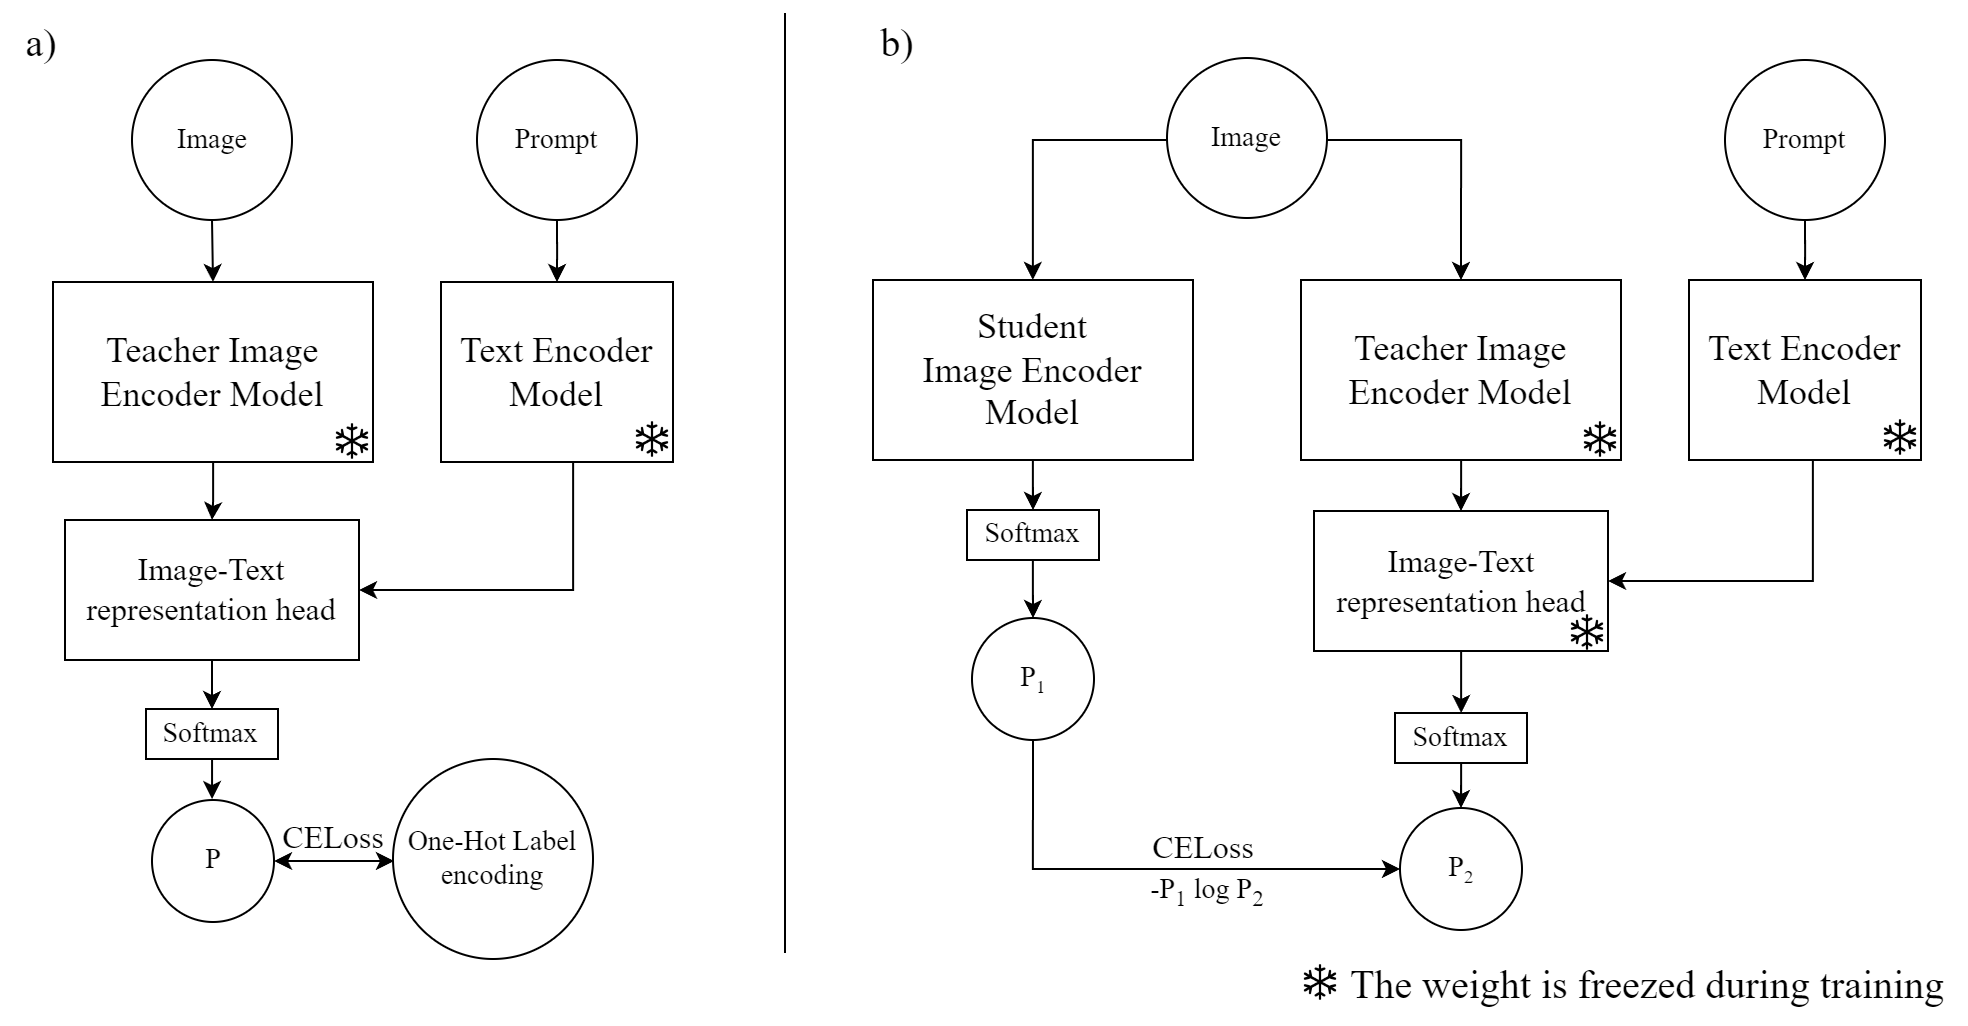
\includegraphics[width=1\textwidth]{Images/Methodology.png}
    \end{center}
    \small a) Training image-text representation head using cross entropy loss b) Self-distillation training by freezing all teacher model
\end{figure}

\begin{figure}[h]
    \caption{Image-Text Cross Attention Classification head}
    \label{fig:cross_attention}
    \centering
    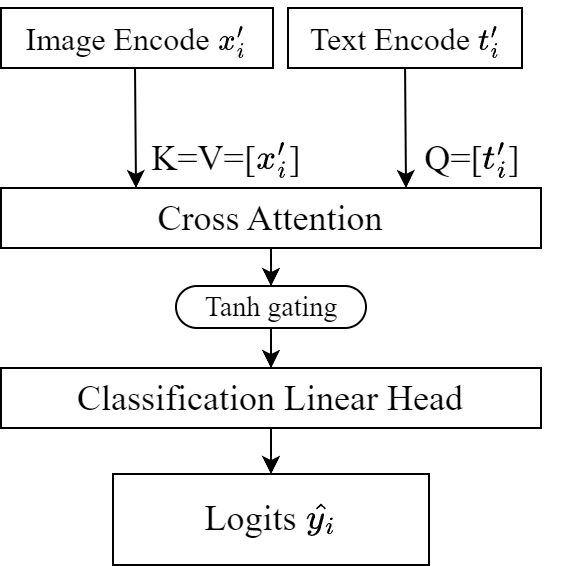
\includegraphics[width=0.5\textwidth]{Images/CrossAttention.png}
\end{figure}

\section{Image-Text Representation Head Training}
% \textcolor{red}{todo:change method image to use sub figure a and b}
In the first step as shown in Figure~\ref{fig:methodology}a), the image-text representation head is trained with image-text pairs $(x_i, t_i)$, where $x_i$ is an $i^{th}$ image input and $t^{th}$ is a $i^{th}$ text created with a propmt ``This is an image of [Class]''.
The teacher image encoder $\theta_{IE}$ and the text encoder $\theta_{TE}$ in the training are pre-trained and freezed.
The image and text encoding are obtained by a mapping function $x'_i = f(x_i; \theta_{IE})$ and $t'_i = f(t_i; \theta_{TE})$ repectively.
The image-text representation head as shown in Figure~\ref{fig:cross_attention} which based on a cross-attention and linear classification layer, is produce logits output as Eq.\ref{eq:cross-attention}.
Then, the logits output from the image-text representation head transform into probability distribution output with a softmax function.

\begin{equation}
    \label{eq:cross-attention}
    \hat{y}_i = \texttt{Softmax}(\texttt{Attention}(K=x'_i, Q=t'_i, V=x'_i))
\end{equation}

The loss function for training the image-text representation head is a cross-entropy as Eq.\ref{eq:loss-cross-attention}, where $y_i\in\{ 0,1 \}^{C}$ is a one-hot encoded label, $C$ is the number of target class and $N$ is the number of training sample.

\begin{equation}
    \label{eq:loss-cross-attention}
    \mathcal{L}_{\texttt{classification}} = -\sum_{i=1}^{N} y_i\log\hat{y}_i
\end{equation}

\section{Self-Distillation}
After the image-text representation head is trained, the image-text representation head is freezed during the self-distillation process.
For the student model, we create a new image encoder model with same architecture as the teacher image encoder model, but with different initialized parameters.
A linear classification and softmax layer is added on top of the student image encoder model to produce output distribution $\hat{s}_i$ for self-distillation process.
The target for training self-distillation is the softmax output $\hat{y}_i$ from image-text representation head with the cross entropy loss as a loss function.
The objective for self-distillation is cross entropy loss as showed in Eq \ref{eq:loss_self_dist}.

\begin{equation}
    \label{eq:loss_self_dist}
    \mathcal{L}_{\texttt{distillation}} = -\sum_{i=1}^{N} \hat{y}_i\log\hat{s}_i
\end{equation}

% \subsection{Teacher student}
% For the teacher model, we will use two stream encoder based model same as CLIP model \shortcite{dosovitskiy2021an}.
% In this experiment, the teacher vision encoder model will be ResNet \shortcite{he2016deep} and ViT \shortcite{dosovitskiy2021an} version.
% For the student model we used the same architecture as teacher vision encoder model, which are ResNet and ViT.
% \textcolor{red}{todo: Add table describes both image and text encoders.}

% \section{Training Objectives}
% In the first step, we trained the image-text representation head with benchmark datasets by using Cross Entropy loss as describe in \ref{fig:overall_method} a). The image and text encoder was freezed during the first step training. For text input, we used "This is the image of [Class]" as a prompt \shortcite{radford2021learning}. After the first image-text representation head were trained, we create a new student model which have the same architecture as a image encoder model with a linear classification head. The student model was randomly initialized parameters. The objective for self-distillation with teacher and student is

\section{Evaluation}
In this work, we evaluate the student model with accuracy using image classification task.
The benchmarks for evalutation are ImageNet, CIFAR-10 and CIFAR-100.
The student model is evaluated compare to the teacher image encoder model using linear probing and student model trained with self-disillation using single image encoder as a teacher model as showed in the Table \ref{tab:experiment_table}.

\begin{table}[h]
    \caption{Experiment evalutation}
    \label{tab:experiment_table}
    \begin{adjustbox}{width=1\textwidth}
        \begin{tabular}{|l|l|l|llll|llll|}
            \hline
            \multirow{2}{*}{\begin{tabular}[c]{@{}l@{}}Teacher Image\\ Encoder\end{tabular}} & \multirow{2}{*}{\begin{tabular}[c]{@{}l@{}}Image Encoder \\ Parameters\end{tabular}} & \multirow{2}{*}{Text Encoder} & \multicolumn{4}{l|}{Self-Distillation without Text} & \multicolumn{4}{l|}{Self-Distillation with Text} \\ \cline{4-11} 
             &  &  & \multicolumn{1}{l|}{CIFAR10} & \multicolumn{1}{l|}{CIFAR100} & \multicolumn{1}{l|}{ImageNet Top1\%} & ImageNet Top5\% & \multicolumn{1}{l|}{CIFAR10} & \multicolumn{1}{l|}{CIFAR100} & \multicolumn{1}{l|}{ImageNet Top1\%} & ImageNet Top5\% \\ \hline
            ViT-B/32 & 86M & RoBERTa & \multicolumn{1}{l|}{} & \multicolumn{1}{l|}{} & \multicolumn{1}{l|}{} &  & \multicolumn{1}{l|}{} & \multicolumn{1}{l|}{} & \multicolumn{1}{l|}{} &  \\ \hline
            ViT-B/32 & 86M & CLIP & \multicolumn{1}{l|}{} & \multicolumn{1}{l|}{} & \multicolumn{1}{l|}{} &  & \multicolumn{1}{l|}{} & \multicolumn{1}{l|}{} & \multicolumn{1}{l|}{} &  \\ \hline
            ViT-B/16 & 86M & RoBERTa & \multicolumn{1}{l|}{} & \multicolumn{1}{l|}{} & \multicolumn{1}{l|}{} &  & \multicolumn{1}{l|}{} & \multicolumn{1}{l|}{} & \multicolumn{1}{l|}{} &  \\ \hline
            ViT-B/16 & 86M & CLIP & \multicolumn{1}{l|}{} & \multicolumn{1}{l|}{} & \multicolumn{1}{l|}{} &  & \multicolumn{1}{l|}{} & \multicolumn{1}{l|}{} & \multicolumn{1}{l|}{} &  \\ \hline
            ResNet-50 & 102M & RoBERTa & \multicolumn{1}{l|}{} & \multicolumn{1}{l|}{} & \multicolumn{1}{l|}{} &  & \multicolumn{1}{l|}{} & \multicolumn{1}{l|}{} & \multicolumn{1}{l|}{} &  \\ \hline
            ResNet-50 & 102M & CLIP & \multicolumn{1}{l|}{} & \multicolumn{1}{l|}{} & \multicolumn{1}{l|}{} &  & \multicolumn{1}{l|}{} & \multicolumn{1}{l|}{} & \multicolumn{1}{l|}{} &  \\ \hline
        \end{tabular}
    \end{adjustbox}
\end{table}

\section{Ablation Study}
\subsection{Few-shot learning}
As this method provides texts for training student image encoder models, the texts provide additional information for better image representations.
Consequently, the student model benefits from our method in few-shot learning situations.
In this part, we provide benchmark results for few-shot learning situations.

\subsection{Using Image captioning as a prompt}
For better understanding the effect of text prompts in our self-distillation method, we experiment by provided better descriptive prompt.
The image captioning model is used to create image description for the self-distillation process.

\subsection{Repeatation self-distillation}
By using student as a teacher model for training another student model, which have the same architecture, but with different initialized parameters.
The performance increased gradually over each generation of the student model \shortcite{furlanello2018born, xie2020self}
In this work, we also investigate the performance increasing over each generation of the student model using our self-distillation method.

\subsection{Image-Text Retrieval}
By the increasing performance in the student model using our method with textual information, we suggest that the student would be a good image encoder which also have information about text.
Such that, we can use our method to improve image-text retrieval task.

% - explainability of the student model like dino or segmentation downstream task. This one aim to test low level semantics information.
% - Repeatation self-distillation like the BornAgain paper.
% - Down stream task with image-text retrieval task.

% \subsection{Error analysis}
% - analysis image task benefit from text which case increase performance and which case not.
% - Few-shot